\documentclass{article}

\usepackage{siunitx}
\usepackage[letterpaper]{geometry}
\usepackage{amsmath}
\usepackage{amssymb}
\usepackage{graphicx}

\def\scriptr{{\mbox{$\resizebox{.09in}{.08in}{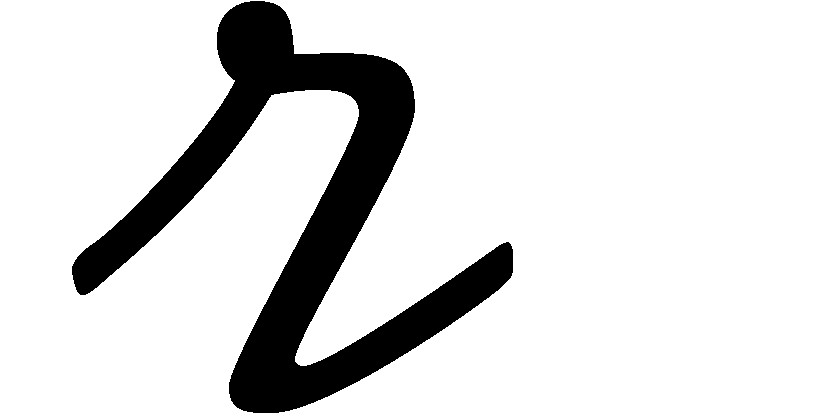
\includegraphics[trim= 1em 0 14em 0,clip]{ScriptR}}$}}}

\title{4132 HW 7}
\author{Duncan Wilkie}
\date{5 April 2022}

\begin{document}

\maketitle

\section*{1a}
Taking the Lorenz gauge,
\[\Box^{2}V=-\frac{1}{\epsilon_{0}}\rho \Rightarrow \rho=0\]
\[
  \Box^{2}\vec{A}--\mu_{0}\vec{J}
  \Rightarrow \nabla^{2}\left( \frac{1}{4\pi\epsilon_{0}}\frac{qt}{r^{2}}\hat{r} \right)-\mu_{0}\epsilon_{0}\frac{\partial^{2}}{\partial t^{2}}\left( \frac{1}{4\pi\epsilon_{0}}\frac{qt}{r^{2}} \right)\hat{r}=-\mu_{0}\vec{J}
\]
\[
  \Rightarrow \frac{1}{r^{2}}\frac{\partial}{\partial r}\left( r^{2}\frac{-1}{2\pi\epsilon_{0}}\frac{qt}{r^{3}}\hat{r} \right)
  -0 = -\mu_{0}\vec{J}
\]
\[
  \Rightarrow -\frac{qt}{2\pi\epsilon_{0}r^{2}}\frac{-1}{r^{2}}\hat{r}=-\mu_{0}\vec{J}
\]
\[
  \Rightarrow \vec{J}=-\frac{qt}{2\pi\epsilon_{0}\mu_{0}r^{4}}\hat{r}
\]

\section*{1b}
Under the given gauge,
\[
  V'=V-\frac{\partial \lambda}{\partial t}
  =\frac{1}{4\pi\epsilon_{0}}\frac{q}{r}
\]
and
\[
  \vec{A}'=\vec{A}+\nabla\lambda
  =\frac{1}{4\pi\epsilon_{0}}\frac{qt}{r^{2}}\hat{r}+\frac{1}{4\pi\epsilon_{0}}\frac{qt}{r^{2}}\hat{r}
  =\frac{1}{2\pi\epsilon_{0}}\frac{qt}{r^{2}}\hat{r}
\]
The first is simply the scalar potential due to a stationary point charge of magnitude $q$,
and the second is radially outward and therefore curl-free, resulting in a zero magnetic field,
also consistent with a stationary point charge.

\section*{2}
Applying the forced wave equation ansatz given in the text,
\[
  \vec{A}(\vec{r},t)=\frac{\mu_{0}}{4\pi}\int_{\mathbb{R}}\frac{J(\vec{r}',t)}{\scriptr}dV
\]
\[
  =\frac{\mu_{0}}{4\pi}\left( \int_{-b}^{-a}\frac{k\left( t-\frac{c}{\scriptr} \right)}{\scriptr}\hat{x}dx
    +\int_{a}^{b}\frac{k\left( t-\frac{c}{\scriptr}\right)}{\scriptr}\hat{x}dx
    +a\int_{0}^{\pi}\frac{k(t-\frac{c}{\scriptr})}{\scriptr}(-\hat{\theta})d\theta
    +b\int_{0}^{2\pi}\frac{k(t-\frac{c}{\scriptr})}{\scriptr}(\hat{\theta})d\theta\right)
\]
The $x$ and $\theta$ dependence of $\scriptr$ may be found from the relation $\scriptr=r-r'=(x)$
% TODO: finish
\section*{3}
The scalar potential is
\[V(\vec{r},t)=\frac{1}{4\pi\epsilon_{0}}\frac{qc}{|\scriptr| c-\scriptr\cdot v}\]
The position of the charge at time $t$ is, in cylindrical coordinates, $r'=a\hat{r}+\omega t\hat{\theta}$.
We may then write
\[\scriptr = {r}-r'=(r-a)\hat{r}+(\theta-\omega t)\hat{\theta}+z\hat{z}\]
The velocity of the charge in cylindrical coordinates is
\[v=\dot{r}\hat{r}+r\dot{\theta}\hat{\theta}+\dot{z}\hat{z}=a\omega\hat{\theta}\]
Plugging this in to the scalar potential,
\[
  V(r,\theta,z,t)=\frac{1}{4\pi\epsilon_{0}}\frac{qc}{a\omega(\omega t-\theta)+c\sqrt{(r-a)^{2}+(\theta-\omega t)^{2}+z^{2}}}
\]
On the $z$-axis, $r=\theta=0$, so
\[V(z,t)=\frac{1}{4\pi\epsilon_{0}}\frac{qc}{at\omega^{2}-c\sqrt{a^{2}+\omega^{2}t^{2}+z^{2}}}\]
The vector potential is
\[
  \vec{A}(\vec{r},t)=\frac{v}{c^{2}}V(\vec{r},t)
  =\frac{a\omega\hat{\theta}}{c^{2}}\frac{1}{4\pi\epsilon_{0}}\frac{qc}{a\omega(\omega t-\theta)
    +c\sqrt{(r-a)^{2}+(\theta-\omega t)^{2}+z^{2}}}
\]
On the $z$-axis, this becomes
\[\vec{A}(z,t)=\frac{1}{4\pi\epsilon_{0}c}\frac{a\omega q}{at\omega^{2}-c\sqrt{a^{2}+\omega^{2}t^{2}+z^{2}}}\hat{\theta}\]

\section*{4}
The Li\'enard-Wiechert potentials are, writing everything in one dimension and applying $\scriptr=r-r'$ with $x'$ as the position of the charge,
\[
  V(x,t)=\frac{1}{4\pi\epsilon_{0}}\frac{qc}{(x-x')c-(x-x')\dot{x}'}
  =\frac{1}{4\pi\epsilon_{0}}\frac{qc}{(c-\dot{x}')(x-x')}
\]
and
\[
  \vec{A}(x,t)=\frac{v}{c^{2}}V(\vec{r},t)
  =\frac{1}{4\pi\epsilon_{0}}\frac{\dot{x}'q}{c(c-\dot{x}')({x-x'})}
\]
Taking the gradient of the first yields
\[
  \vec{E}(x,t)=-\frac{qc}{4\pi\epsilon_{0}(c-\dot{x})}\frac{1}{(x-x')^{2}}\hat{x}
  =\frac{1}{4\pi\epsilon_{0}}\frac{-qc}{c-v}\frac{1}{\scriptr^{2}}
\]
Taking the

\end{document}

%%% Local Variables:
%%% mode: latex
%%% TeX-master: t
%%% End:
